\documentclass[12pt]{extreport}

\usepackage[utf8]{inputenc}
\usepackage{setspace}
\usepackage{graphicx}

\onehalfspacing

% Title Page
\title{A Multiagent Approach to Autonomous Intersection Management}
\author{Alperen Karen\\Mateusz Nowotyński}


\begin{document}
\maketitle

\chapter{The Problem}
Once autonomous vehicles become popular, autonomous interactions amongst multiple vehicles will be possible. Current methods of vehicle coordination, which are all designed to work with human drivers, will be outdated. The bottleneck for roadway efficiency will no longer be the drivers, but rather the mechanism by which those drivers’ actions are coordinated. While open-road driving is a well-studied and more-or-less-solved problem, urban traffic scenarios, especially intersections, are much more challenging.

Existing intersection control schemes, such as traffic signals or stop signs, must conform to human behavioral limitations and are highly inefficient. By contrast, AVs communicating with reservation-based intersection managers can make much better use of available roadway capacity, reducing delay by up to two orders of magnitude at highly congested intersections.

\chapter{Proposed solution}
In our solution we have two types of agents. One is intersection manager which have full authority over the intersection. Second one is car agent that represents car approaching intersection. When car comes close to the intersection he sends request to the intersection agent containing his speed, estimated time of arrival, dimensions, desired direction and on which lane he is approaching. In the response he receives rejection or approval containing path to follow. When car receives rejection then he slows down and retries later.

Intersection agent store the intersection in form of spatially and temporally discreet grid. On receiving request he generates possible path of the car and check for conflicts. In cases of conflict he sends rejection, otherwise marks time slots as reserved and sends path to the car.

\begin{figure}
	\begin{center}
		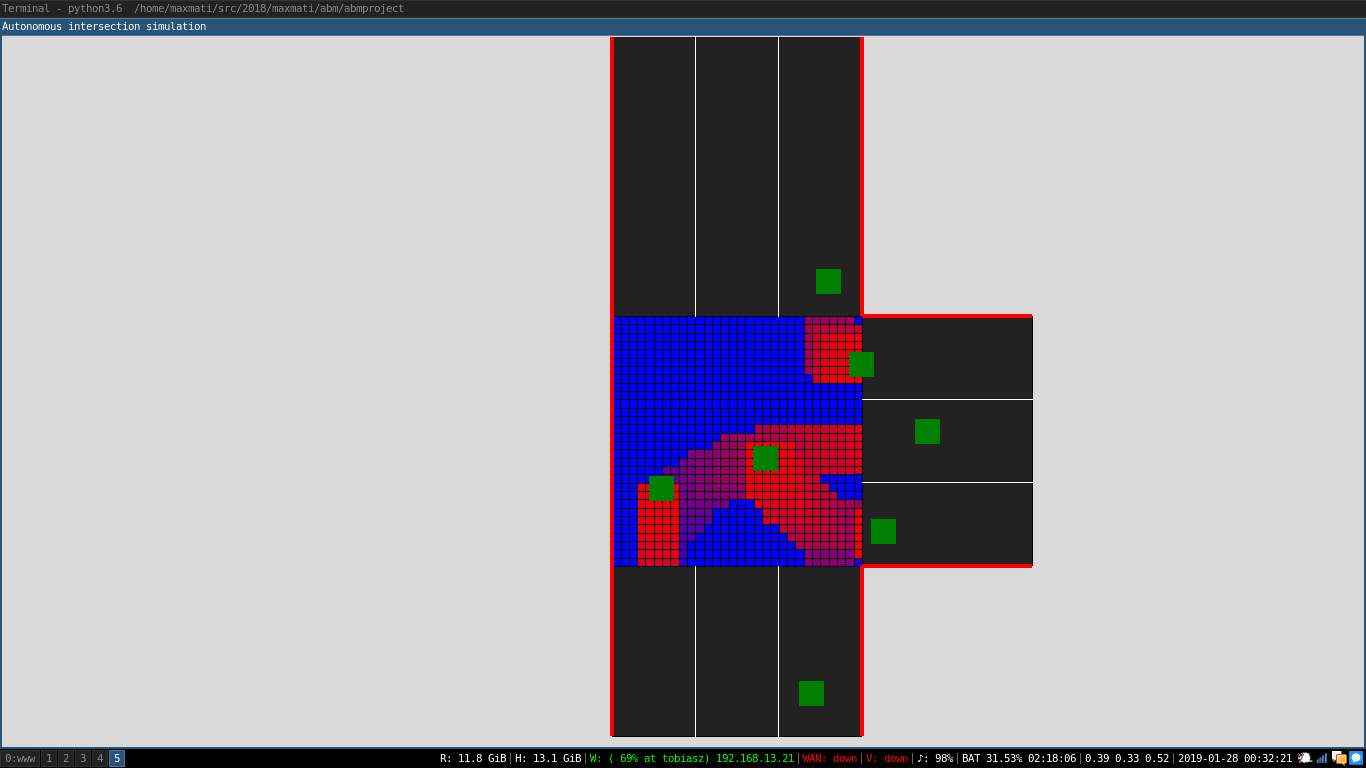
\includegraphics[width=\linewidth]{screnshot}
	\end{center} 
	\caption{Sample intersection simulation}
\end{figure}

  


\chapter{Coparasion with real case}
During implementation of problem solving algorithm, real life traffic situation of Kawiory intersection is compared with our solution output. In contrast we did not propose traffic light in the simulation, we had much better traffic flow performance. Real intersection had flow of 30 cars per minute, in our simulation we achieved 85 cars a minute.

\end{document}          
